\changecolours{ScoutGreen}
\section[Expressões e Árvores]{Expressões Compostas e Árvores de Consulta}

% ------------------------------------------------------------------------------
\twocolframe[title={Construção de Consultas Algébricas Complexas},leftcol=7.0cm,rightcol=7.0cm]{%
  \alert{Estratégia 1: Expressão Única Aninhada}\par
  \itemseps[topsepi=0.5mm,itemsepi=1mm,labelsep=2mm,leftmargini=3mm]
  \begin{itemize}
    \item Graças ao princípio de Fechamento Relacional, operadores podem ser encadeados diretamente:
      \[ \boldsymbol{\pi_{\text{titulo, preco}}\left(\sigma_{\text{cat} = '\text{Lit.}' \,\land\, \text{preco} < 50}(\text{LIVRO})\right)} \]
    \item Avaliação da expressão é feita de dentro para fora (dos parênteses mais internos para os externos).
    \item Concisa, mas pode se tornar densa em consultas de grande porte.
  \end{itemize}
}{%
  \alert{Estratégia 2: Variáveis Intermediárias ($\leftarrow$)}\par
  \itemseps[topsepi=0.5mm,itemsepi=1mm,labelsep=2mm,leftmargini=3mm]
  \begin{itemize}
    \item Divide o problema em etapas lógicas lineares:
      {\footnotesize
      \begin{align*}
        \text{LIT} &\leftarrow \sigma_{\text{cat} = '\text{Lit.}'}(\text{LIVRO}) \\
        \text{BARATOS} &\leftarrow \sigma_{\text{preco} < 50}(\text{LIT}) \\
        \text{RES} &\leftarrow \pi_{\text{titulo, preco}}(\text{BARATOS})
      \end{align*}}
    \item Extremamente clara para depuração didática e documentação de passos analíticos.
  \end{itemize}
}

% ------------------------------------------------------------------------------
\twocolframe[title={Árvores de Consulta Relacional (Query Trees)},leftcol=6.5cm,rightcol=7.5cm]{%
  \alert{Estrutura e Avaliação Hierárquica}\par
  \itemseps[topsepi=0.5mm,itemsepi=1mm,labelsep=2mm,leftmargini=3mm]
  \begin{itemize}
    \item É a estrutura interna utilizada pelos SGBDs para planejar consultas.
    \item \textbf{Folhas (Base):} Relações físicas armazenadas em disco.
    \item \textbf{Nós Internos:} Operadores algébricos ($\sigma, \pi, \times, \dots$).
    \item \textbf{Raiz (Topo):} Relação final resultante entregue ao usuário.
    \item \textbf{Execução Bottom-Up:} Os dados sobem das folhas em direção à raiz.
  \end{itemize}
}{%
  \alert{Visualização da Árvore de Consulta}\par
  \vspace{1mm}
  \centering
  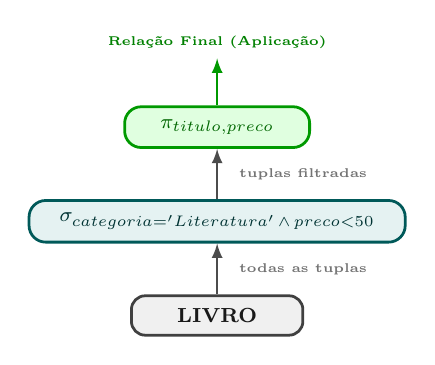
\begin{tikzpicture}[
    scale=0.92,
    every node/.style={transform shape},
    rootnode/.style={
      rectangle, rounded corners=6pt,
      draw=green!60!black, fill=green!12,
      text=green!40!black, font=\bfseries\footnotesize,
      inner xsep=14pt, inner ysep=5pt, align=center,
      line width=1pt
    },
    opnode/.style={
      rectangle, rounded corners=6pt,
      draw=teal!70!black, fill=teal!10,
      text=teal!40!black, font=\bfseries\footnotesize,
      inner xsep=12pt, inner ysep=5pt, align=center,
      line width=1pt
    },
    relnode/.style={
      rectangle, rounded corners=5pt,
      draw=black!75, fill=black!6,
      text=black!90, font=\bfseries\footnotesize,
      inner xsep=18pt, inner ysep=5pt, align=center,
      line width=1pt
    },
    edge label/.style={
      font=\tiny\bfseries, text=black!55, right=5pt, align=left
    }
  ]
    % Nós da árvore (com espaçamento vertical equilibrado e sem sobreposição)
    \node[rootnode] (proj) at (0, 2.6) {$\pi_{\text{titulo, preco}}$};
    \node[opnode]   (sel)  at (0, 1.3) {$\sigma_{\text{categoria} = '\text{Literatura}' \,\land\, \text{preco} < 50}$};
    \node[relnode]  (base) at (0, 0)   {LIVRO};

    % Conexões direcionadas Bottom-Up
    \draw[->, thick, >=latex, draw=black!70] (base.north) -- (sel.south)
      node[midway, edge label] {todas as tuplas};

    \draw[->, thick, >=latex, draw=black!70] (sel.north) -- (proj.south)
      node[midway, edge label] {tuplas filtradas};

    \draw[->, thick, >=latex, draw=green!60!black] (proj.north) -- ++(0, 0.65cm)
      node[above, font=\bfseries\tiny, text=green!50!black] {Relação Final (Aplicação)};
  \end{tikzpicture}
}

% ------------------------------------------------------------------------------
\twocolframe[title={Heurística Fundamental: Empurrar Seleções para Baixo},leftcol=7.0cm,rightcol=7.0cm]{%
  \alert{O Princípio de Otimização}\par
  \itemseps[topsepi=0.5mm,itemsepi=1mm,labelsep=2mm,leftmargini=3mm]
  \begin{itemize}
    \item Em consultas complexas envolvendo produtos cartesianos ou uniões, a ordem das operações impacta drasticamente o desempenho.
    \item \textbf{Regra de Ouro (Push-Down Selection):}\\
      Aplicar as operações de seleção ($\sigma$) o mais cedo possível na árvore (o mais próximo das folhas).
    \item Filtrar antes de cruzar reduz a quantidade de tuplas em memória RAM.
  \end{itemize}
}{%
  \alert{Comparativo de Custo Computacional}\par
  \itemseps[topsepi=0.5mm,itemsepi=1mm,labelsep=2mm,leftmargini=3mm]
  \begin{itemize}
    \item \textbf{Plano Ingênuo:}\\
      $\sigma_{\text{cond}}(R \times S)$\\
      Primeiro gera todas as $10.000 \times 10.000 = 100.000.000$ linhas do produto cartesiano para depois filtrar.
    \item \textbf{Plano Otimizado:}\\
      $(\sigma_{\text{condR}}(R)) \times (\sigma_{\text{condS}}(S))$\\
      Reduz $R$ para $10$ linhas e $S$ para $5$ linhas, gerando um produto de apenas $50$ linhas!
  \end{itemize}
}
